% Основной текст отчёта: постановка задачи, реализация, результаты

\section{Постановка задачи}
Интерполяционным сплайном третьей степени называется функция, удовлетворяющая следующим условиям:
\begin{enumerate}
    \item На каждом отрезке $[x_{i-1}, x_i]$ совпадает с некоторым многочленом третьей степени.
    \item Проходит через заданные узлы $S(x_i) = y_i$.
    \item Непрерывна на отрезке $[x_0, x_n]$ со всеми своими производными до второго порядка включительно (такая функция образует сплайн дефекта 1).
\end{enumerate}

Для частичного отрезка $[x_i, x_{i+1}]$ сплайн определяется интерполяционной формулой Эрмита:
\[
S_i(x) = y_i + m_i(x - x_i) + c_i(x - x_i)^2 + d_i(x - x_i)^3
\]
Необходимые наклоны $m_i$ находятся из решения системы линейных алгебраических уравнений (СЛАУ), которая дополняется граничными условиями. В данной работе применяются односторонние разностные производные в крайних узлах. Значения мантисс вычисляются с точностью до 4 знаков.

Функция $y = f(x)$ задана таблицей 1.
\begin{table}[h]
\centering
\begin{tabular}{|c|ccccccccc|}
\hline
$x_i$ & 0.100 & 0.210 & 0.295 & 0.348 & 0.419 & 0.475 & 0.511 & 0.555 & 0.609 \\
$y_i$ & 0.0010 & 0.0441 & 0.0868 & 0.1205 & 0.1738 & 0.2219 & 0.2554 & 0.2988 & 0.0002 \\
\hline
\end{tabular}
\caption{Исходные данные}
\end{table}

\section{Реализация и проведение расчетов}
\subsection{Чтение данных и инициализация шагов}
Шаги интерполяции $h_i = x_{i+1} - x_i$:
\begin{itemize}
    \item $h_0 = 0.1100$
    \item $h_1 = 0.0850$
    \item $h_2 = 0.0530$
    \item $h_3 = 0.0710$
    \item $h_4 = 0.0560$
    \item $h_5 = 0.0360$
    \item $h_6 = 0.0440$
    \item $h_7 = 0.0540$
\end{itemize}

\begin{lstlisting}[language=Python]
import numpy as np
import matplotlib.pyplot as plt

# Исходные данные
x = np.array([0.100, 0.210, 0.295, 0.348, 0.419, 0.475, 0.511, 0.555, 0.609])
y = np.array([0.0010, 0.0441, 0.0868, 0.1205, 0.1738, 0.2219, 0.2554, 0.2988, 0.0002])
n = len(x)
h = np.diff(x)
\end{lstlisting}

\subsection{Граничные условия}
Граничные условия для производных $m_0$ и $m_n$, вычисленные как односторонние разностные производные:
\begingroup
\large
\begin{align*}
m_0 &= \frac{y_1 - y_0}{h_0} = 0.3918 \\
m_n &= \frac{y_n - y_{n-1}}{h_{n-1}} = -5.5296
\end{align*}
\endgroup

\begin{lstlisting}[language=Python]
m0 = (y[1] - y[0]) / h[0]
mn = (y[-1] - y[-2]) / h[-1]
\end{lstlisting}

\subsection{Составление и решение СЛАУ}
Уравнения для внутренних узлов выводятся из условия непрерывности второй производной $S''_{i-1}(x_i) = S''_i(x_i)$. Для каждого $i$ (от $1$ до $n-2$):
\[
a_i m_{i-1} + 2m_i + b_i m_{i+1} = c_i
\]
Уравнения образуют трехдиагональную матрицу. В результате решения системы получены вектора $m_i$ в узлах сплайна (с точностью до 4 знаков):
\begin{itemize}
    \item $m_0 = 0.3918$
    \item $m_1 = 0.4300$
    \item $m_2 = 0.5881$
    \item $m_3 = 0.6695$
    \item $m_4 = 0.8871$
    \item $m_5 = 0.6515$
    \item $m_6 = 1.7372$
    \item $m_7 = -2.1460$
    \item $m_8 = -5.5296$
\end{itemize}

\begin{lstlisting}[language=Python]
A = np.zeros((n, n))
b = np.zeros(n)

A[0, 0] = 1.0; b[0] = m0
A[-1, -1] = 1.0; b[-1] = mn

for i in range(1, n-1):
    a_i = h[i] / (h[i-1] + h[i])
    b_i = h[i-1] / (h[i-1] + h[i])
    c_i = 3*a_i*((y[i]-y[i-1])/h[i-1]) + 3*b_i*((y[i+1]-y[i])/h[i])

    A[i, i-1] = a_i; A[i, i] = 2.0; A[i, i+1] = b_i
    b[i] = c_i

m = np.linalg.solve(A, b)
\end{lstlisting}

\section{Кубические сплайны на отрезках}
Искомые формулы кубического сплайна на участках вычисляются напрямую из $m$ и $y$ :
\begingroup
\large
\begin{align*}
S_0(x) &= 0.0010 + 0.3918(x - 0.100) - 0.3469(x - 0.100)^2 + 3.1537(x - 0.100)^3 \\
S_1(x) &= 0.0441 + 0.4300(x - 0.210) + 0.6938(x - 0.210)^2 + 1.8547(x - 0.210)^3 \\
S_2(x) &= 0.0868 + 0.5881(x - 0.295) + 1.1668(x - 0.295)^2 - 5.0255(x - 0.295)^3 \\
S_3(x) &= 0.1205 + 0.6695(x - 0.348) + 0.3677(x - 0.348)^2 + 10.9391(x - 0.348)^3 \\
S_4(x) &= 0.1738 + 0.8871(x - 0.419) + 2.6977(x - 0.419)^2 - 57.1563(x - 0.419)^3 \\
S_5(x) &= 0.2219 + 0.6515(x - 0.475) - 6.9045(x - 0.475)^2 + 407.1008(x - 0.475)^3 \\
S_6(x) &= 0.2554 + 1.7372(x - 0.511) + 37.0623(x - 0.511)^2 - 1230.1532(x - 0.511)^3 \\
S_7(x) &= 0.2988 - 2.1460(x - 0.555) - 125.3179(x - 0.555)^2 + 1160.3508(x - 0.555)^3
\end{align*}
\endgroup

\begin{lstlisting}[language=Python]
coeffs_a, coeffs_b, coeffs_c, coeffs_d = [], [], [], []
for i in range(n-1):
    dy = y[i+1] - y[i]
    coeffs_a.append(y[i])
    coeffs_b.append(m[i])
    coeffs_c.append((3*dy/(h[i]**2)) - (2*m[i]+m[i+1])/h[i])
    coeffs_d.append((-2*dy/(h[i]**3)) + (m[i]+m[i+1])/(h[i]**2))
\end{lstlisting}

\section{Результаты и графики}
Итоговый график склейки полученных кубических сплайнов:
\begin{figure}[H]
    \centering
    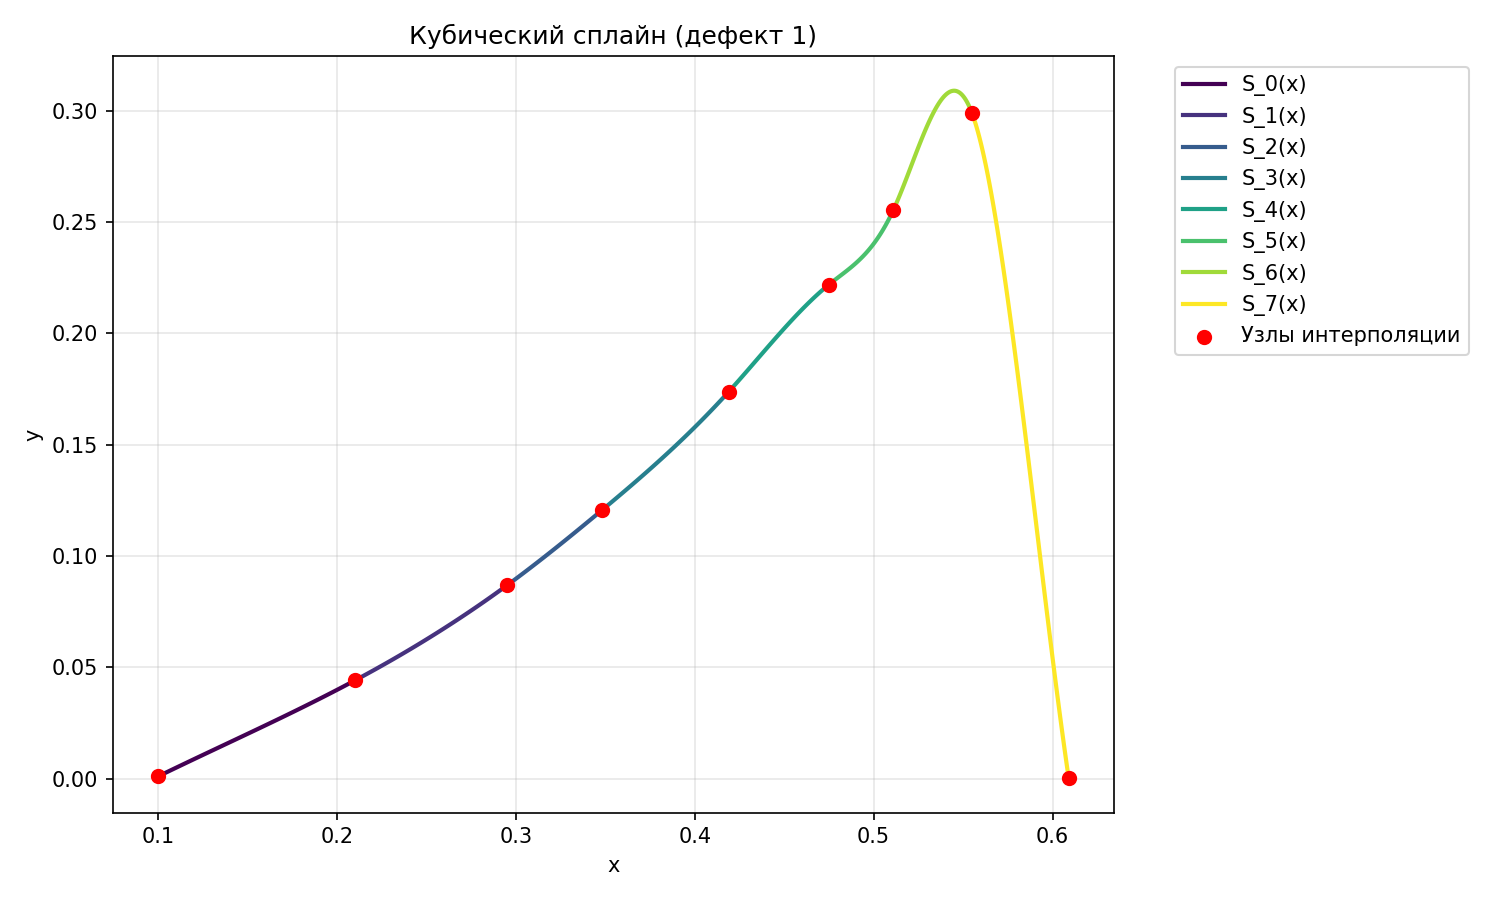
\includegraphics[width=0.9\textwidth]{pct/spline.png}
    \caption{Кубический сплайн дефекта 1}
    \label{fig:spline}
\end{figure}

\section{Проверка условий налагаемых на сплайн}
Необходимо проверить условия сшивки сплайнов в промежуточных узлах $x_i$, $i=1 \dots n-1$. Сплайн должен удовлетворять условиям $C^2$-гладкости:
$S_{left}(x_i) = S_{right}(x_i)$, $S'_{left}(x_i) = S'_{right}(x_i)$ и $S''_{left}(x_i) = S''_{right}(x_i)$. Вычислим значения левых и правых пределов для каждого узла:

\textbf{В узле $x_1 = 0.210$:}
\begin{itemize}
    \item $S_{left} = 0.0441, \quad S_{right} = 0.0441 \quad | \Delta \approx 6.9e-18$
    \item $S'_{left} = 0.4300, \quad S'_{right} = 0.4300 \quad | \Delta \approx 3.3e-16$
    \item $S''_{left} = 1.3876, \quad S''_{right} = 1.3876 \quad | \Delta \approx 2.7e-15$
\end{itemize}
\textbf{В узле $x_2 = 0.295$:}
\begin{itemize}
    \item $S_{left} = 0.0868, \quad S_{right} = 0.0868 \quad | \Delta \approx 1.4e-17$
    \item $S'_{left} = 0.5881, \quad S'_{right} = 0.5881 \quad | \Delta \approx 3.3e-16$
    \item $S''_{left} = 2.3335, \quad S''_{right} = 2.3335 \quad | \Delta \approx 6.2e-15$
\end{itemize}
\textbf{В узле $x_3 = 0.348$:}
\begin{itemize}
    \item $S_{left} = 0.1205, \quad S_{right} = 0.1205 \quad | \Delta \approx 1.4e-17$
    \item $S'_{left} = 0.6695, \quad S'_{right} = 0.6695 \quad | \Delta \approx 6.7e-16$
    \item $S''_{left} = 0.7354, \quad S''_{right} = 0.7354 \quad | \Delta \approx 1.5e-14$
\end{itemize}
\textbf{В узле $x_4 = 0.419$:}
\begin{itemize}
    \item $S_{left} = 0.1738, \quad S_{right} = 0.1738 \quad | \Delta \approx 0.0e+00$
    \item $S'_{left} = 0.8871, \quad S'_{right} = 0.8871 \quad | \Delta \approx 0.0e+00$
    \item $S''_{left} = 5.3954, \quad S''_{right} = 5.3954 \quad | \Delta \approx 3.6e-14$
\end{itemize}
\textbf{В узле $x_5 = 0.475$:}
\begin{itemize}
    \item $S_{left} = 0.2219, \quad S_{right} = 0.2219 \quad | \Delta \approx 2.8e-17$
    \item $S'_{left} = 0.6515, \quad S'_{right} = 0.6515 \quad | \Delta \approx 1.0e-15$
    \item $S''_{left} = -13.8091, \quad S''_{right} = -13.8091 \quad | \Delta \approx 4.3e-14$
\end{itemize}
\textbf{В узле $x_6 = 0.511$:}
\begin{itemize}
    \item $S_{left} = 0.2554, \quad S_{right} = 0.2554 \quad | \Delta \approx 0.0e+00$
    \item $S'_{left} = 1.7372, \quad S'_{right} = 1.7372 \quad | \Delta \approx 0.0e+00$
    \item $S''_{left} = 74.1247, \quad S''_{right} = 74.1247 \quad | \Delta \approx 0.0e+00$
\end{itemize}
\textbf{В узле $x_7 = 0.555$:}
\begin{itemize}
    \item $S_{left} = 0.2988, \quad S_{right} = 0.2988 \quad | \Delta \approx 5.6e-17$
    \item $S'_{left} = -2.1460, \quad S'_{right} = -2.1460 \quad | \Delta \approx 4.4e-16$
    \item $S''_{left} = -250.6358, \quad S''_{right} = -250.6358 \quad | \Delta \approx 1.1e-13$
\end{itemize}

\section{Заключение}
Все условия, налагаемые на кубический сплайн дефекта 1, успешно проверены аппаратно: значения на концах участков совпадают, а также доказана непрерывность функции, её первой и второй производных. Смещения левых и правых пределов во внутренних узлах стремятся к машинному нулю (от $10^{-15}$ до $10^{-17}$). Таким образом, полученные функции гладко сопрягаются и образуют полноценную $C^2$-сплайн-аппроксимацию.
